\documentclass{article}

%............Inicia Preambulo.......................
\usepackage{graphicx}
\usepackage{float}
\usepackage[utf8]{inputenc}
\usepackage[shortlabels]{enumitem}
\usepackage{textcomp}
\usepackage{multicol}
\usepackage{caption}
\usepackage[spanish]{babel}
\usepackage[total={17.5cm, 23cm}, top=2cm, left=2cm]{geometry}
\usepackage{esvect}
\usepackage[font=footnotesize]{caption}

\spanishdecimal{.}
\parindent 0cm

%.............Fin de Preambulo........................

\begin{document}

\begin{center}
{\Large \textbf{Universidad Autónoma de Coahuila}}
\end{center}

\begin{center}
{\large Facultad de Ciencias Físico-Matemáticas}
\end{center}

%Materia
\begin{center}
{\large Metodos Numericos}
\end{center}

%Título
\begin{center}
{\large Biseccion}
\end{center}

%Fecha
\begin{center}
{\large 29 de Noviembre del 2019}
\end{center}

%Autor
\begin{center}
{\large José Antonio Olveda García}
\end{center}

\vspace{5mm}

\begin{multicols}{2}
\section{Objetivo}
\label{sec:Obj}
Explicar uno de los metodos de buscadores de raices mas sencillos para asi dar introduccion, a los metodos de buscadores de raices mas complejos. 

\section{Introduccion}
\label{sec:Intro}
El método de bisección es un algoritmo de búsqueda de raíces que trabaja dividiendo el intervalo a la mitad y seleccionando el subintervalo que tiene la raíz.
\section{Metodologia}
\label{sec:Met}
Este método consiste en obtener una mejor aproximación de la raíz a partir de un intervalo inicial (a,b) en el cual hay un cambio de signo en la función, es decir: $f(a)f(b)<0$.

Se obtiene el punto medio:
\begin{equation}
X_{m}=\frac{a+b}{2}
\end{equation}
donde $x_{m}$ es la nueva aproximación a  la raíz, y se vuelve a tomar un intervalo, pero ahora mas pequeño, considerando que siga existiendo un cambio de signo en la función, es decir, el nuevo intervalo queda determinado por:
\\
El método termina cuando se cumple con alguna condición de paro, en este programa la condición es la tolerancia :
\\
\begin{equation}
E_{a}=|V_{R}-V{E}|
\end{equation}
Sin embargo a pesar de que la formula de encuentra el error absoluto establecido entre los puntos, el valor de este no es tan preciso, es por eso que para el calculo de errores se recomienda el uso de la siguiente formula
\begin{equation}
E_{a}=\frac{P_{m0}+P_{m}}{P_{m0}-P_{m}}
\end{equation}
y la formula del error relativo comunmente esta proporcionada por la siguiente formula 
\begin{equation}
E_{r}=\frac{V_{R}-V_{E}}{V_{R}} (100)
\end{equation}
Sin embargo al igual que la formula anterior establecida, esta no es totalmente exacta, debido a esto se debe de tomar en una mayor consideracion a la formula siguiente
\begin{equation}
E_{r}=Er=\frac{P_{m0}-P_{m}}{P_{m0}}
\end{equation}
Este es un método “de encierro”, para aplicarlo se debe contar con un intervalo inicial, en donde f(a)*f(b) < 0. Este método requiere de menos pasos en un programa, sin embargo converge mas lentamente que el de Newton-Raphson.

Los pasos del método son los siguientes: 

1.- Localizar un intervalo que contenga al menos una raíz.

2.- Dividir el intervalo en dos partes iguales reteniendo la mitad en donde f(x) cambia de signo, para conservar al menos una raíz.

3.- Repetir el procesó varias veces hasta cumplir con la tolerancia deseada.


si $f(m) f(b)<0$ entonces conservar (m,b) como el sem. intervalo que contiene al menos una raíz.

A cada paso se le llama “iteración”  y reduce el intervalo a la mitad.

Después de cada iteración el intervalo se reduce a la mitad, después de $n$ iteraciones, el intervalo original se había reducido $2^{n}$ veces, por lo tanto, si el intervalo original  es de tamaño $a$ y el criterio de convergencia aplicado al valor absoluto de la diferencia de dos $X_{m}$ consecutivas es  $ \epsilon $, entonces se requerían $n$ iteraciones donde $n$ se calcula con la igualdad de la expresión:
\begin{equation}
\frac{a}{2^{n}} \leq \epsilon
\end{equation}
de donde $n=\frac{\log a - \log \epsilon}{\log 2} $
\section{Ejemplos}
\label{sec:Ejem}
Ejemplo1

Buscar la raíz de$ x^{5} - x + 3  = 0 $

    $f (-2) = (-2)^{5} - (-2) + 3 = -32 + 2 + 3 = -27  $       es negativo

    $f (-1) = (-2)^5 - (-1) + 3 = -1 + 1 + 3 = 3 $         es positivo
\\
\\
Debe haber por lo menos una raíz en (-2,-1)  

                        t = -1.5

$f (-1.5) = (-1.5)^{5} - (-1.5) + 3 = - 7.59 + 1.3 + 3 = -3.09375$ negativo

El intervalo donde cambia el signo es

     (-1.5,-1)

\begin{center}
$X_{m}=\frac{-1.5-1}{2}=-1.25$
\end{center}
	

    $ f (-1.25) = (-1.25)^5 - (-1.25) + 3 = -3.0 + 1.25 + 3 = 1.19824 $ positivo



La raíz “R” esta en el intervalo (-1.5,-1.25)

\begin{center}
$X_{m}=\frac{-1.5-1.25}{2}=-1.375$
\end{center} 

$f (-1.375)^2 = (-1.375)^5 - (-1.375) + 3 = -0.5398 $ negativo

Hay que determinar un numero máximo de iteraciones

Normalmente esto se hace considerando una “tolerancia” , esto es:

El valor absoluto de la diferencia de la  $x_{i+1}-x_{i}$ debe ser menor que la tolerancia o el resultado de alguna fórmula de error debe ser menor que la tolerancia dada.

Una de las fórmulas de error mas útiles es la del error relativo porcentual aproximado: 
\begin{center}
        $ E_{r}=Er=\frac{P_{m0}-P_{m}}{P_{m0}}$
\end{center}
Ventajas: este método se aplica a cualquier función continua y no requiere derivadas 

Desventajas: es un método lento 

Una de las limitaciones de este método es que puede resultar un polo considerándolo como un “cero” ,por ejemplo, la sig. función tiene un cambio de signo cerca del origen.
\\
En este caso, nunca se va a encontrar una raíz, aunque haya un cambio de signo en la función en el intervalo dado.

\section{Ventajas y Desventajas}
\label{sec:Ven}
\textbf{Ventajas}
\\
1. Es siempre convergerte 
\\
2. Es optimo para resolver una ecuacion f (x)=0 cuando no se sabe nada de f, excepto calcular su signo.
\\
3. Requiere que f sea continua en el intervalo especificado
\\
4. Se basa en el Teorema de Bolzano
\\
5. Se puede establecer el limite de error.
\\
6. Es facil de implementar.
\\
\\
\textbf{Desventajas}
\\
1. Converge muy lentamente 
\\
2. Permite encontrar solo una raiz, aunque existan mas en el intervalo.
\\
3. Algunas veces la determinacion del intervalo inicial no es muy facil
\\
4. A veces, no es obvio el criterio de finalizacion del proceso iteractivo.
\\
5. No puede determinar  raices complejas.
\\
6. Es dificil generalizando para dimensiones superiores.



\section{Implementacion del programa}
\label{sec:Imp}
El programa genera la aproximacion de raices por medio del metodo de biseccion a partir de las ecuaciones mostradas anteriormente, añadiendo un adicional de la grafica de la funcion deseada, esto con el objetivo de dar a entender al usuario que es lo que esta sucediendo ahi, cabe mencionar que los criterios del metodo de biseccion tambien estan presentes y son escenciales para la resolucion de estos, en este caso el ejemplo para mostrar el funcionamiento de la funcion deseada es de $x^3-5$ evaluada en el intervalo $[0,2]$ con un error de $E=0.0001$, mostrando asi una tabla donde muestra los datos sobre mis puntos a, b y el punto medio que se encontracion en la $n$ iteracion, asi como la funcion evaluada en el punto medio de la funcion misma, el error relativo y el error absoluto a partir de mis formulas estimadas de la forma mas precisa (veanse las ecuaciones 3 y 5)
\begin{figure}[H]
\centering
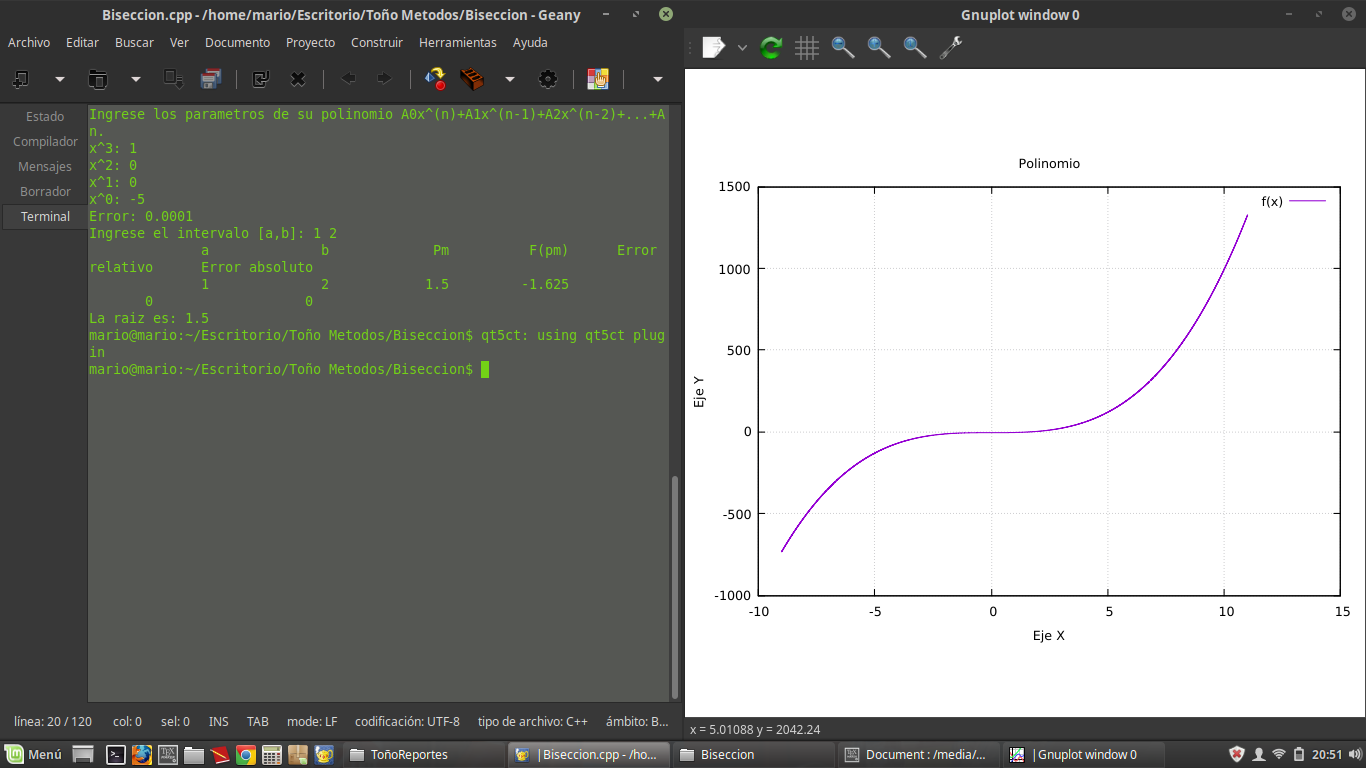
\includegraphics[scale=.125]{Biseccion.png}
\caption{Metodo de Biseccion programado}
\end{figure}
Como podemos apreciar la raiz de la funcion implementada en mi programa es correcta por lo que el metodo de bisecion funcionaria siemre y cuando cumpla con los terminos designados de los productos de mis funciones evaluadas en mis puntos, de lo contrario no podra obtener una raiz, debido a que si este criterio no se cumple, por lo tanto no podra ejecutarse el programa.



\end{multicols}

\end{document}